\clearpage
\setcounter{page}{1}

\begin{center}
\title{\LARGE \bf Mengenal Python dan Anaconda}
\end{center}

\appendix
\section{Teori}

\section*{\normalsize 1. Sejarah dan Perbedaan}

\hspace {\parindent} Python diciptakan pertama kali oleh Guido Van Rossum di Centrum Wiskunde and Informatica (CWI) di belanda awal tahun 1990. Nama bahasa pemrograman ini diambil dari nama grup komedi di Inggris yang digemari oleh Guido yaitu "Monty Python". 

Bahasa Pemrograman ini terinspirasi dari bahasa pemrograman ABC. Python bersifat open source. Open source berarti bahasa ini masih dapat dikembangkan oleh orang lain yang ingin mengembangkannya.

Guido lanjut membuat bahasa python ini di Corporation for \textit{National Research Initiative} (CNRI) di Amerika pada tahun 1995. Pada pembuatan ini kemudian rilis beberapa versi Python. 

Kemudian, Guido dan tim developer Python-nya pindah ke BeOpen.com pada tahun 2000 dan kemudian mereka membuat tim BeOpen PythonLabs. Kemudian timnya pindah ke Digital Creation yang saat ini menjadi perusahaan "Zope". 

Pada tahun 2001, mereka membentuk Organisasi Python yang bernama \textit{Python Software Foundation} (PSF). PSF merupakan organisasi yang dibuat khusus untuk hak intelektual Python.

Setelah dirilis, python memiliki beberapa versi. Setiap versi memiliki perbedaan, berikut adalah perbedaan python versi 2 dan versi 3:
\begin{enumerate}[label=\alph*.]

\item Syntax untuk mencetak teks\\
Pada python 2 untuk menuliskan perintah cetak tidak harus menggunakan kurung tetapi menggunakan kurung juga bisa. Contoh:\\
print "gini juga bisa"\\
Sedangkan pada python 3, mencetak harus disertai kurung.  Contoh:\\
print ("kalo gasalah mah gini hehe")

\item Syntax untuk mencetak teks\\
Pada python 2 untuk menuliskan perintah input user menggunakan perintah raw\textunderscore input. Contoh:\\
nama = raw\textunderscore input('masukin apa ajaa')\\
Sedangkan pada python 3,  perintah input user menggunakan perintah input.  Contoh:\\
nama = input('masukin apa ajaa')\\

\item Hasil dari operator pembagian\\
Pada python 2 jika dituliskan code :\\
print "3 / 2 = " , 3/2\\
print "3 // 2 = " , 3//2\\
print "3 / 2.0 = " , 3/2.0\\
print "3 // 2.0 = " , 3//2.0\\

maka akan dihasilkan 

3 / 2 = 1\\
3 // 2 = 1\\
3 / 2.0 = 1.5\\
3// 2.0 = 1.0\\

sedangkan pada python 3 akan menghasilkan 

3 / 2 = 1.5\\
3 // 2 = 1\\
3 / 2.0 = 1.5\\
3// 2.0 = 1.0\\

\end{enumerate}

\section*{\normalsize 2. Implementasi Penggunaan Python pada Perusahaan Dunia}
\hspace {\parindent} Salah satu perusahaan besar pengguna python adalah perusahaan google. Python menjadi bahasa yang digunakan pada Google App Engine.Google menggunakan pemrograman python untuk webnya dengan menggunakan library python, tools, dan framework. Programmer pada google menggunakan python untuk membangun sistem administrasi, Format package internal google, dan aplikasi penampil kode. Selain itu, python digunakan juga pada platform youtube. Penggunaan python pada youtube digunakan untuk menampillkan video, mengontrol template websitenya, dan mengakses data data. 

%SECTION 2 --------------------------------------------------------------------------<<<<

\section{Instalasi}
\begin{enumerate}

\item Instalasi Python

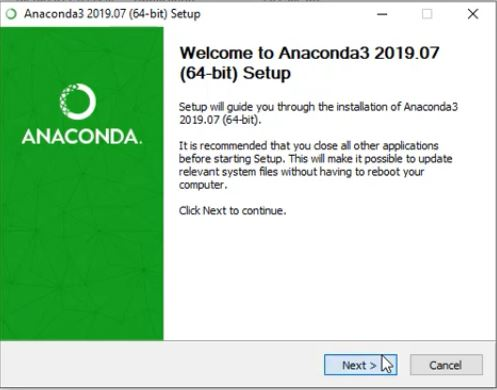
\includegraphics{gambar/1_1.jpg}
Klik Next\\

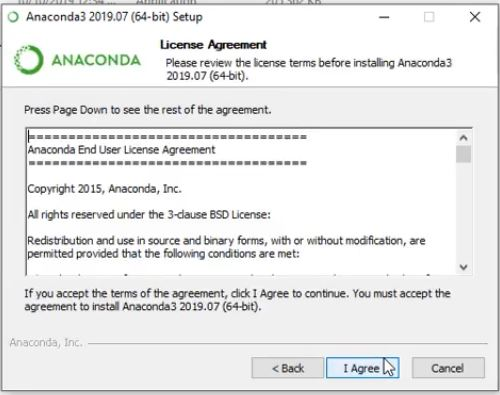
\includegraphics{gambar/1_2.jpg}
Klik agree untuk menyetujui\\

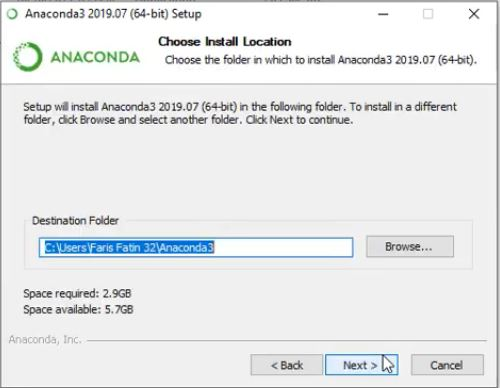
\includegraphics{gambar/1_3.jpg}
Pilih Direktori Instalasi\\

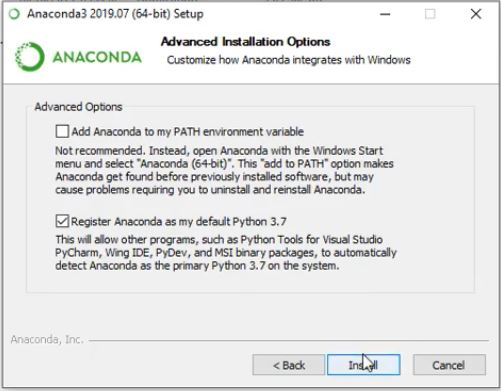
\includegraphics{gambar/1_4.jpg}
Klik Install\\

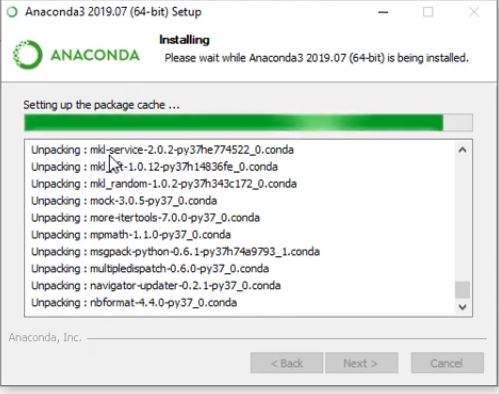
\includegraphics{gambar/1_5.jpg}
Tunggu Instalasi selesai\\

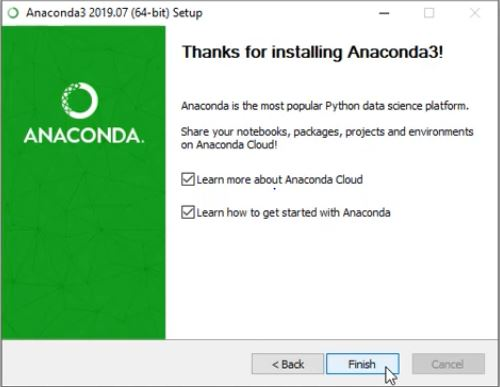
\includegraphics{gambar/1_6.jpg}
Instalasi Selesai\\

Link Video Instalasi:\\
https://www.youtube.com/watch?v=FK9Nw4udNXo

\item Instalasi pip

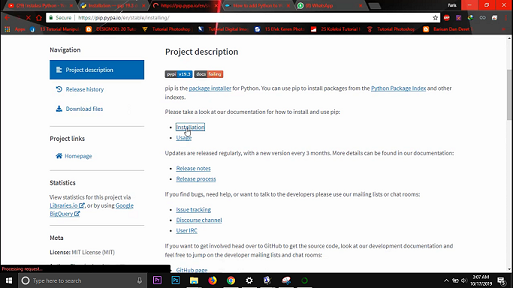
\includegraphics{gambar/2_1.png}
Buka website pip.py\\

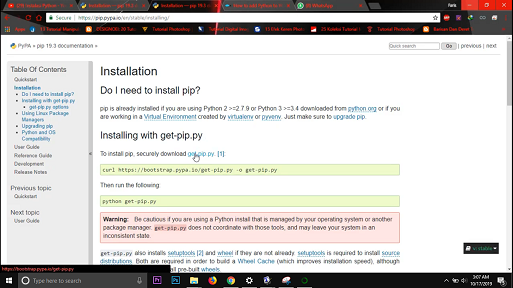
\includegraphics{gambar/2_2.png}
Klik file get-pip.py\\

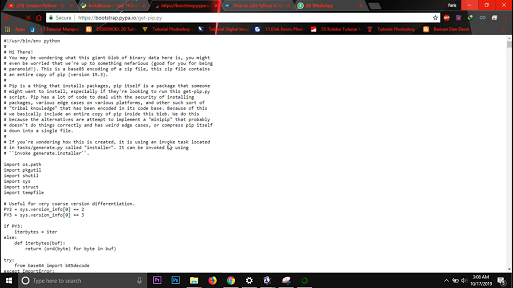
\includegraphics{gambar/2_3.png}
Download file get-pip.py ke pc anda\\

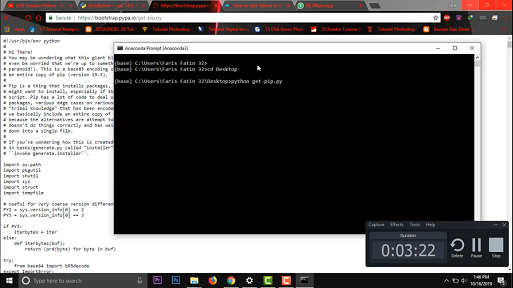
\includegraphics{gambar/2_4.png}
Buka cmd dan ketikan perintah "python get-pip.py" dan tunggu hingga instalasi berjalan\\

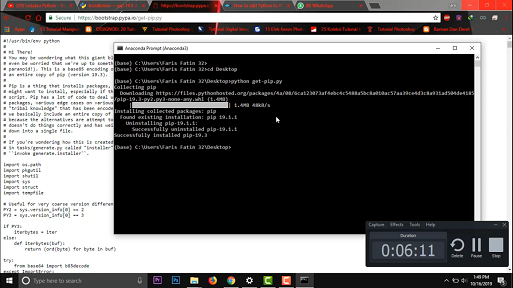
\includegraphics{gambar/2_5.png}
Instalasi Selesai.\\

Link Video Instalasi: \\
https://www.youtube.com/watch?v=IY8JATmTJWA

\item Cara setting environtment 

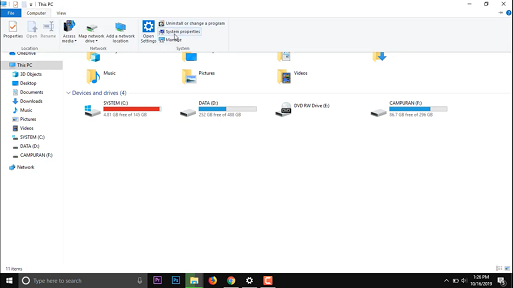
\includegraphics{gambar/3_1.png}
Buka system properties kalian di windows\\

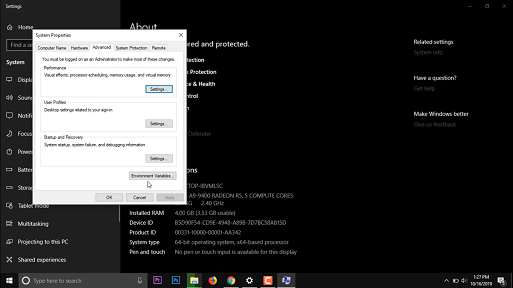
\includegraphics{gambar/3_2.png}
Buka advance system setting\\

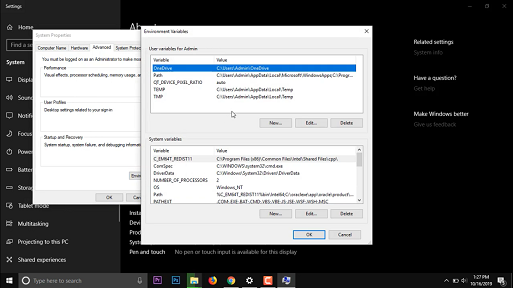
\includegraphics{gambar/3_3.png}
Klik environtment variables\\

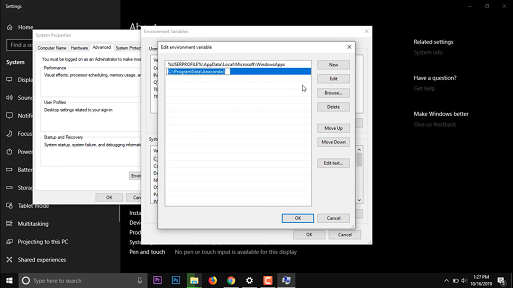
\includegraphics{gambar/3_4.png}
Pilih environtment path python.\\

Link Video Cara Setting Environment: \\
https://www.youtube.com/watch?v=K0MbX8limL0

\item Mencoba enterpreter CLI melalui Windows

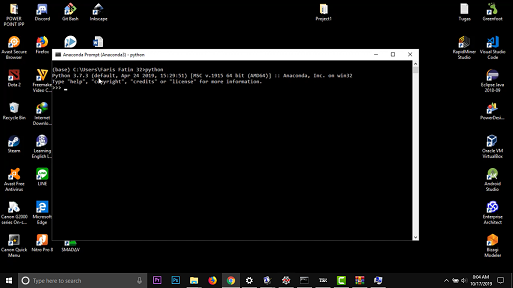
\includegraphics{gambar/4_1.png}
Buka CLI/ Command prompt\\

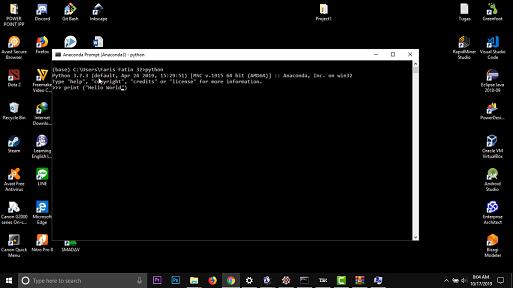
\includegraphics{gambar/4_2.png}
Ketikkan perintah yang akan digunakan.  Contoh: print("Hello World")\\

Link Mencoba Interpreter CLI: \\
https://www.youtube.com/watch?v=bLlsRxhst2k

\item Menjalankan dan mengupdate anaconda spyder

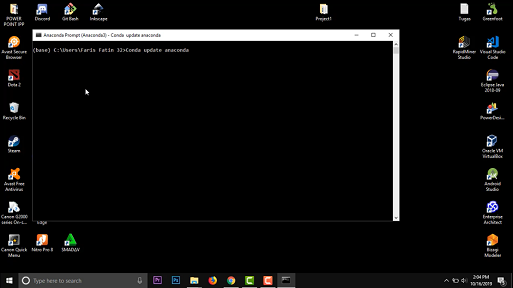
\includegraphics{gambar/5_1.png}
Buka CLI/ Command Prompt. Kemudian ketikan "conda update anaconda"'\\

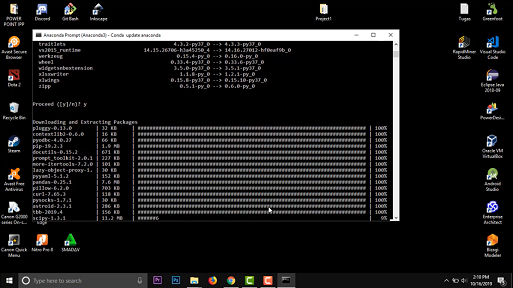
\includegraphics{gambar/5_2.png}
conda akan otomatis mendownload dan mengupdate anaconda.\\

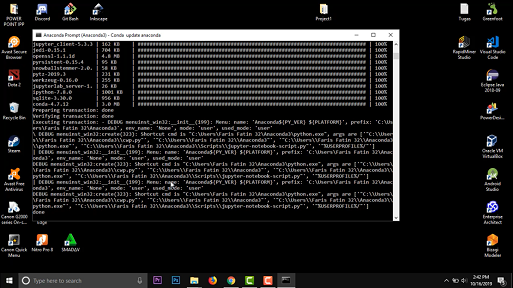
\includegraphics{gambar/5_3.png}
Update selesai\\

Link Video Menjalankan dan Mengupdate Anaconda Spyder: \\
https://www.youtube.com/watch?v=gwLwTYvgPUI

\item Cara menjalankan script hello world di spyder

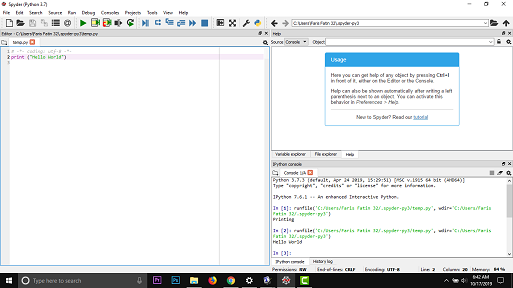
\includegraphics{gambar/6_1.png}
Ketikkan print("Hello World") dan kemudian di run, maka hasil akan muncul di kolom console\\

Link Video Menjalankan Script Hello World di Spyder: \\
https://www.youtube.com/watch?v=IlOn\textunderscore9oV35k

\item Cara menjalankan Script otomatis login aplikasi akademik dengan library selenium dan inputan user

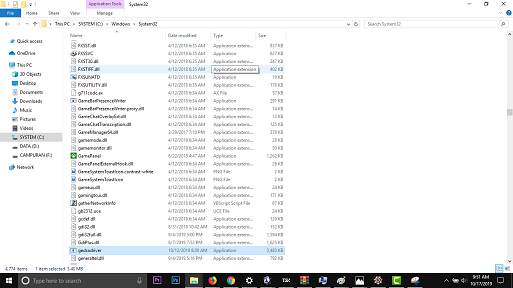
\includegraphics{gambar/7_1.png}
Download dan copy driver browser ke system 32\\
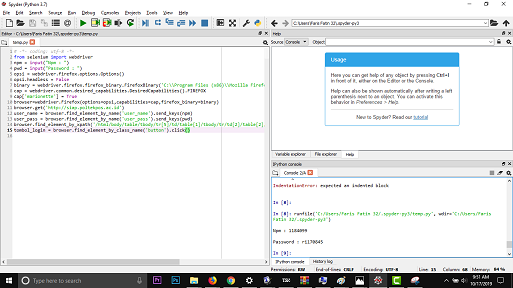
\includegraphics{gambar/7_2.png}
Tuliskan Script seperti pada gambar\\
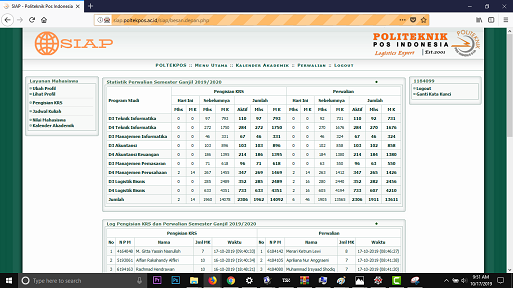
\includegraphics{gambar/7_3.png}
Berhasil login secara otomatis.

\item Cara menggunakan variable explorer di spyder

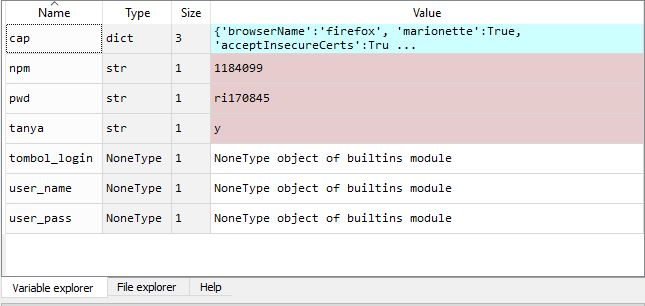
\includegraphics{gambar/8_1.jpg}
Variable explorer dihgunakan untuk mencari apa saja nama, type, dan value dari variable yang digunakan pada spyder. Variable explorer bisa digunakan untuk mengedit dan mengubah variable.

\end{enumerate}

\section {Identasi}
\begin{enumerate}
\item Pengertian
Indentasi adalah penulisan paragraf yang menjorok kedalam. Bahasa pemrograman python mengunakan identasi sebagai tatacara menulis dan tidak menggunakan tanda kurung lagi.

\item {Jenis Jenis error}

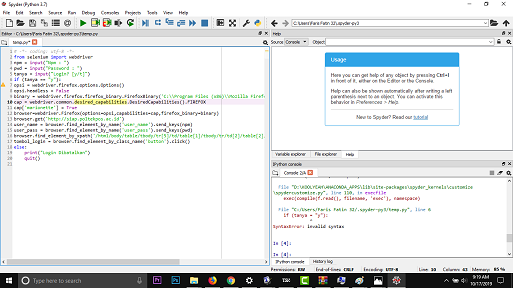
\includegraphics{gambar/identasi1}
Error disini disebabkan karena indentasi yang kurang benar pada pemrograman python. 


\item {Cara membaca Error}

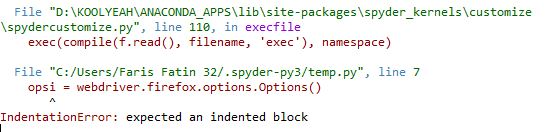
\includegraphics{gambar/identasi3.jpg}
opsi = webdriver.firefox.options.Options() berarti ada error di bagian ini.\\
IndentationError: expected an indented block berarti error pada line tadi disebabkan oleh identasi\\


\item{Cara Menangani Error}

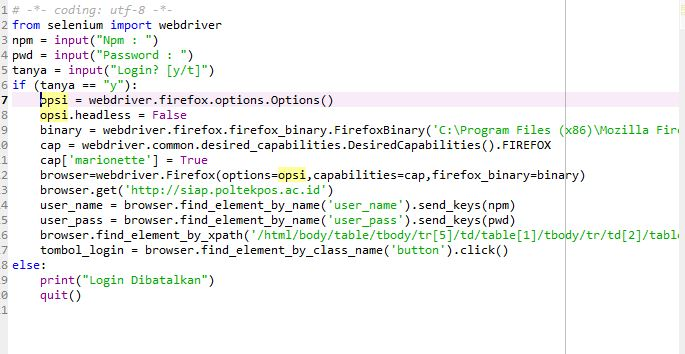
\includegraphics{gambar/identasi4.jpg}
Cara menangani errornya dengan mmeberikan indentasi ke line yang belum terindentasi.\\
\end{enumerate}







